\PassOptionsToPackage{unicode=true}{hyperref} % options for packages loaded elsewhere
\PassOptionsToPackage{hyphens}{url}
%
\documentclass[]{book}
\usepackage{lmodern}
\usepackage{amssymb,amsmath}
\usepackage{ifxetex,ifluatex}
\usepackage{fixltx2e} % provides \textsubscript
\ifnum 0\ifxetex 1\fi\ifluatex 1\fi=0 % if pdftex
  \usepackage[T1]{fontenc}
  \usepackage[utf8]{inputenc}
  \usepackage{textcomp} % provides euro and other symbols
\else % if luatex or xelatex
  \usepackage{unicode-math}
  \defaultfontfeatures{Ligatures=TeX,Scale=MatchLowercase}
\fi
% use upquote if available, for straight quotes in verbatim environments
\IfFileExists{upquote.sty}{\usepackage{upquote}}{}
% use microtype if available
\IfFileExists{microtype.sty}{%
\usepackage[]{microtype}
\UseMicrotypeSet[protrusion]{basicmath} % disable protrusion for tt fonts
}{}
\IfFileExists{parskip.sty}{%
\usepackage{parskip}
}{% else
\setlength{\parindent}{0pt}
\setlength{\parskip}{6pt plus 2pt minus 1pt}
}
\usepackage{hyperref}
\hypersetup{
            pdftitle={BASS4 - ADMINISTRATOR'S MANUAL},
            pdfauthor={Louise Serenhov, Erik Sjöstrand, Jenny-Li Örsell \& Brjánn Ljótsson},
            pdfborder={0 0 0},
            breaklinks=true}
\urlstyle{same}  % don't use monospace font for urls
\usepackage{longtable,booktabs}
% Fix footnotes in tables (requires footnote package)
\IfFileExists{footnote.sty}{\usepackage{footnote}\makesavenoteenv{longtable}}{}
\usepackage{graphicx,grffile}
\makeatletter
\def\maxwidth{\ifdim\Gin@nat@width>\linewidth\linewidth\else\Gin@nat@width\fi}
\def\maxheight{\ifdim\Gin@nat@height>\textheight\textheight\else\Gin@nat@height\fi}
\makeatother
% Scale images if necessary, so that they will not overflow the page
% margins by default, and it is still possible to overwrite the defaults
% using explicit options in \includegraphics[width, height, ...]{}
\setkeys{Gin}{width=\maxwidth,height=\maxheight,keepaspectratio}
\setlength{\emergencystretch}{3em}  % prevent overfull lines
\providecommand{\tightlist}{%
  \setlength{\itemsep}{0pt}\setlength{\parskip}{0pt}}
\setcounter{secnumdepth}{5}
% Redefines (sub)paragraphs to behave more like sections
\ifx\paragraph\undefined\else
\let\oldparagraph\paragraph
\renewcommand{\paragraph}[1]{\oldparagraph{#1}\mbox{}}
\fi
\ifx\subparagraph\undefined\else
\let\oldsubparagraph\subparagraph
\renewcommand{\subparagraph}[1]{\oldsubparagraph{#1}\mbox{}}
\fi

% set default figure placement to htbp
\makeatletter
\def\fps@figure{htbp}
\makeatother

\usepackage{booktabs}
\usepackage{amsthm}
\makeatletter
\def\thm@space@setup{%
  \thm@preskip=8pt plus 2pt minus 4pt
  \thm@postskip=\thm@preskip
}
\makeatother
\usepackage[]{natbib}
\bibliographystyle{apalike}

\title{BASS4 - ADMINISTRATOR'S MANUAL}
\author{Louise Serenhov, Erik Sjöstrand, Jenny-Li Örsell \& Brjánn Ljótsson}
\date{Last updated 2020-07-08}

\begin{document}
\maketitle

{
\setcounter{tocdepth}{1}
\tableofcontents
}
\hypertarget{introduction}{%
\chapter{Introduction}\label{introduction}}

BASS is a flexible tool for creating online psychological treatment programs.
In this manual you will learn how to manage participants, combine self-help material into treatments, keep track on events during an ongoing study/program, manage security and privacy settings, collect and export data and communicate with participants through the administration interface of BASS.

\hypertarget{dictionary}{%
\chapter{Dictionary}\label{dictionary}}

These are recurrent concepts in the manual:

\textbf{Instrument}
An instrument is an electronic version of a paper form used during psychological assessment. Some examples of digitalized instruments are VAS (visual analogue scale), MADRS (Montgomery Åsberg Depression Rating Scale), SWLS (Satisfaction With Life Scale) and LSAS (Liebowitz Social Anxiety Scale).

\textbf{Assessment}
An assessment is a set of instruments, given in a specific order and at a specific occasion or for a specific number of occasions. A pre- and post-treatment assessment often consist of the same instruments with the afterward addition of one instrument measuring treatment satisfaction.

\textbf{Type}
A type represents the time-aspect of an assessment. Each assessment is linked to a type, typically SCREEN, PRE, POST or FOLLOW-UP or a customized type.

\textbf{Project}
A project is the administrative concept that connects a set of assessments to a set of participants.

\textbf{Participants}
A participant need to be assigned to a project to be able to fill in instruments and follow an assessment.

\textbf{Group}
A project can be divided into groups, and participants of the same group in a project can be managed collectively.

\hypertarget{login}{%
\chapter{Login}\label{login}}

As soon as your database setup is ready, you can login to the administrator's interface. The interface is found at an URL of the format ``\url{https://webcbt.se/NameOfYourDatabase}''. Enter your credentials in the login box and press the Login button.

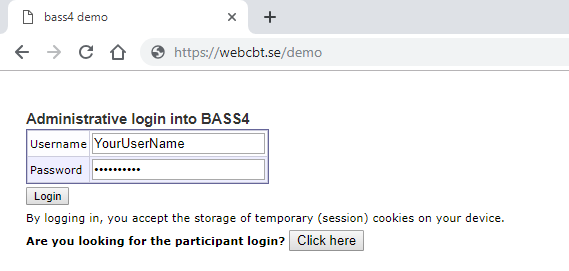
\includegraphics{images/login.png}

\hypertarget{the-main-menu}{%
\chapter{The main menu}\label{the-main-menu}}

All functionality in the BASS administration interface can be accessed from the main menu to the left of your screen.

Which options are visible in the main menu depends on your authorization level. A usual setup is that one administrator manages the available instruments and assessments, while several therapists manage their own participants and individual treatments.

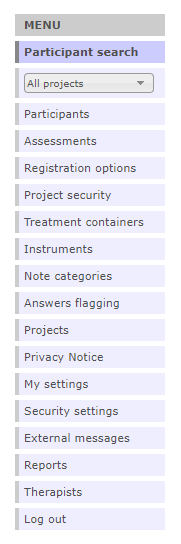
\includegraphics{images/main-menu.png}

\hypertarget{search-participants}{%
\chapter{Search participants}\label{search-participants}}

The ``Participant search'' is located at the top of the main menu. This is where you can search for and list participants by specific variables such as groups or projects.

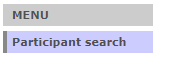
\includegraphics{images/search-participants-menu.png}

When you press ``Participant search'' you will see a view with four tabs:

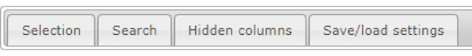
\includegraphics{images/search-participants-tab.png}

\begin{itemize}
\tightlist
\item
  Selection -- Add a filter to your search
\item
  Search -- Perform your search using text strings or other identifiers
\item
  Hidden columns -- View and show columns that are hidden
\item
  Save/load settings -- Save your recurrent searches for convenience
\end{itemize}

\hypertarget{selectionfilter}{%
\section{Selection/filter}\label{selectionfilter}}

If you press Selection, you can add a filter to your participant search.

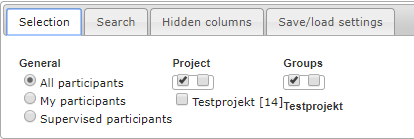
\includegraphics{images/selection-filter.png}

Here you can choose if you want to search all participants, your own participants (that you treat) or participants whose treatments you supervise.

You can also choose which project(s) or group(s) to search. The top two checkboxes can be used to quickly either mark or unmark all the below listed projects or groups. If no specific project or group is checked, all of them will be included in the search. This also means that unchecking all projects/groups won't return participants without a project/group.

\begin{quote}
\textbf{Hint:} If you want to search a specific group you should only mark that group, and not the corresponding project, as this will return all the participants belonging to the project and not only those in the group.
\end{quote}

Your chosen selection of participants is shown in the participant list below the tab.

\hypertarget{search}{%
\section{Search}\label{search}}

The actual search is done in the \textbf{Search} tab. If you previously added search filters in the Selection tab they will now be active and delimit your search.

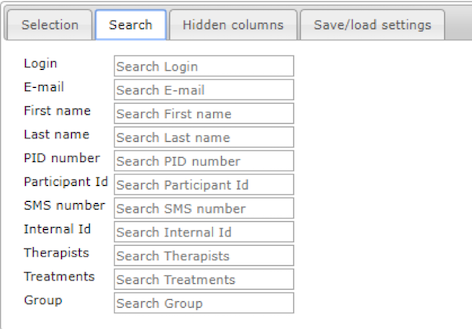
\includegraphics{images/search.png}

Here you can use many different variables to search for one or several participants. The search is executed either automatically when you leave a filled-in search box or when you hit the Enter-key on your keyboard. Your search results are shown in the participant list below the tab.

Note that there is a discrepancy when searching by numbers or by text strings:

\begin{itemize}
\item
  Searching for the number ``12'' will only show the exact hit, while adding a \% sign to the search as in ``12\%'' will return both ``12'', ``123'' and ``012''.
\item
  Searching for the text string ``my'' will return both ``My'', ``Myra'' and ``Amy''. You don't need to add any \% sign for text string searches.
\end{itemize}

To search for several participants at the same time, you add a space between each corresponding search term in the search box.

\begin{quote}
\textbf{Hint:} This is useful if you want to search for participants whose IDs are listed on different rows in an Excel-file. Just copy the ID containing rows in Excel and directly paste them into the search box in BASS and they automatically receive a space between them.
\end{quote}

\hypertarget{hide-show-and-sort-columns}{%
\section{Hide, show and sort columns}\label{hide-show-and-sort-columns}}

If you want to hide a column, you hover the mouse over the column header until a red X shows up. By pressing the X, the column will be hidden.

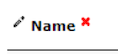
\includegraphics{images/hide-show-sort.png}

To show/unhide a column, press the ``Hidden columns'' tab. This tab shows all hidden columns as buttons. Press the button with the column you want back and it will show up in the search results again.

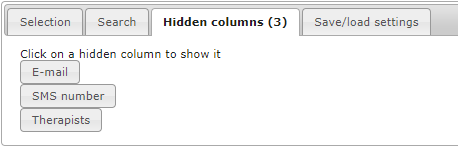
\includegraphics{images/hidden-columns.png}

Most columns can be sorted alphabetically or by number. To sort a column, press the small up/down arrows that show when you hover over the column header.

\hypertarget{column-explanations}{%
\section{Column explanations}\label{column-explanations}}

There are a number of columns showing information, status or possible actions for a participant. Some are explained in the table below.

Column

Description

Pen symbol

Edit the participant

Participant Id

A unique identifier for a participant within the study/project. ``ANX-001''

Internal Id

A unique and technical identifier for a participant within the database.

Flag symbol

Shows if the participant is flagged for something.

Message symbol

Shows if there are unread messages from the participant.

Chat symbol

(For supervised therapists)
Shows if there are unread messages from the supervisor.

Approval symbol

(For supervisors)
Shows if there are messages sent from a supervised therapist to a participant that might need approval.

Superv Mess

(For supervisors)
Total number of messages in supervisory correspondence. This is a useful way to see how much guidance was needed from the supervisor.

Last message

Last date when a participant sent a message (was active). Sort on this column and you'll find participants that are lagging behind.

Weeks

The number of weeks left of the treatment.
Treatments without end date are marked with the eternity symbol.

Module

The latest module the participant got access to. This column also shows for how many days the participant has had access to the module.

Homework

Shows if there is an unread homework sent in by the participant.

Group

Shows which group a participant belongs to. You can change the group here, but you need to save the update with the Save button below the list.

Heart symbol

By pressing the heart, you add the participant to your participants.

Trash symbol

By pressing the trash symbol, you delete the participant. Be careful as the participant and all its corresponding data then will be lost.

\hypertarget{saveload-search-settings}{%
\section{Save/load search settings}\label{saveload-search-settings}}

To save your current search settings, including both filters and search parameters, press the Save/load settings-tab. First ensure that the current search result for the settings you want to save are shown in the table below. Then write a name for your settings in the Currently loaded settings box and press ``Save as new''.

\begin{quote}
\textbf{Hint:} Be careful to not use the ``Save'' button instead, because this will overwrite any currently loaded settings including its name.
\end{quote}

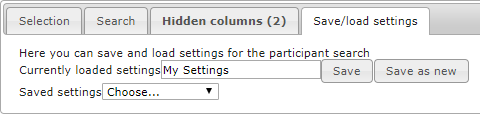
\includegraphics{images/save-load1.png}

The text ``saved!'' appears to the right of the buttons and your search is now saved and available in the dropdown below.

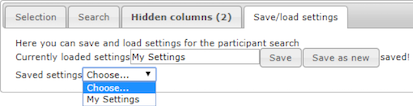
\includegraphics{images/save-load2.png}

The dropdown ``Saved settings'' is where you access all your previously saved search settings.

\begin{quote}
\textbf{Hint:} If you make a new search, the ``Currently loaded settings'' box may no longer reflect the content of the search result list below. To be sure that the list matches the settings you want to load, first select ``Choose'' in the dropdown menu and then reselect the settings you want.
\end{quote}

\hypertarget{add-new-participant-to-group-and-change-group}{%
\subsection{ADD NEW PARTICIPANT TO GROUP AND CHANGE GROUP}\label{add-new-participant-to-group-and-change-group}}

It is possible to directly create a new participant within a specific project. This function is found below the table of participants. Just choose which project you want to add the new participant to, and you will be redirected to the ``New participant''-view with this project pre-filled.

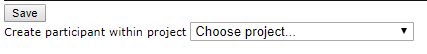
\includegraphics{images/add-new-participants.png}

It is also easy to change which group a participant belongs to. For each participant in the table, you can choose a project in the dropdown in the Group column. Don't forget to save all changes by pressing the ``Save'' button below the table afterwards.

\hypertarget{assessments}{%
\chapter{Assessments}\label{assessments}}

Assessments are accessed from the ``Assessments'' option in the main menu. Note that you first have to choose a project in the dropdown in the main menu to make the Assessments option for that project visible. When you press ``Assessments'' you will see a view showing the existing assessments of the chosen project. All assessments that are listed in this view can be manually sorted with the upwards pointing arrow symbols to the right of each assessment name.

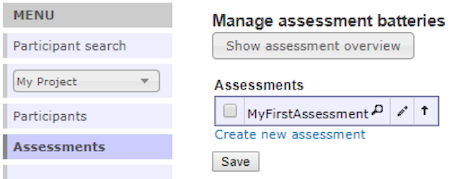
\includegraphics{images/assessement.png}

You can show or hide the expanded overview by pressing the Show assessments overview-button. Here you can get a quick review of all the included assessments and their corresponding attributes.

\textbf{Hint:} Among other things, the assessment overview shows the order of each instrument in all assessments. This is a good place to ensure that the instrument order is kept from one assessment to another throughout the project. It also enables you to easily see if you somewhere have missed to include an instrument that should appear in several, similar assessments.

\hypertarget{create-or-edit-assessments}{%
\section{Create or edit assessments}\label{create-or-edit-assessments}}

Add a new assessment to your project by pressing ``Create new assessment'' at the bottom of the Assessment view. To instead edit an existing assessment, press the pencil symbol to the right of the name of the assessment you want to edit. This opens up the assessment panel where you can set a number of variables that define the assessment:

\hypertarget{name}{%
\subsection{Name}\label{name}}

Here you can fill in a name for your assessment, for example \textbf{\emph{Screening}}.

\hypertarget{labelcustom-label}{%
\subsection{Label/Custom label}\label{labelcustom-label}}

You can either select one of the predefined labels in the drop-down, or write your own label in the Custom label textbox. Adding a custom label will surpass any predefined label that is selected from the drop-down. Note that the assessment label will be visible in reports when you export your data.

\begin{quote}
\textbf{Hint:} By selecting Weekly-assessment or Point-assessment some stats for Repetition (below) are preset.
\end{quote}

\hypertarget{managed}{%
\subsection{Managed}\label{managed}}

This option sets whether data-gathering is managed individually or in groups.

\begin{quote}
\textbf{Hint:} If you have different cohorts, you may want to choose In group. Screening assessments are usually managed In group and these can be activated or deactivated for a certain group and date under Participants -\textgreater{} Groups -\textgreater{} screening group name -\textgreater{} Show -\textgreater{} Assessments.
\end{quote}

\begin{quote}
\textbf{Hint:} If your participants start their treatments at different times, you usually choose Individually. The Individually option is also more flexible for long-term studies spanning over months when participants go for vacation and need some individual adjustment to the timing of assessments.
\end{quote}

\hypertarget{repitition}{%
\subsection{Repitition}\label{repitition}}

The Repetition option sets if the assessment is to be done once or repeatedly, and if so at what intervals and for how many times.

Assessments with the predefined label ``Weekly'' have repetition set to Weekly and the interval to 7 days.

Assessments with the label ``Point-assessment'' have repetition set to Manual. This means that the next assessment can be set manually to occur at an arbitrary date, independent of the time of the previous assessment. This is useful for assessments that are triggered by irregular events, for example a major flair of symptoms.

\hypertarget{time-limit}{%
\subsection{Time limit}\label{time-limit}}

Here you can set if participants have to fill out the assessment within a certain time limit.

\begin{quote}
\textbf{Important note:} Setting a time limit for an assessment is extremely important to prevent the results being mixed up with those from similar, subsequent assessments. For example, if an ongoing POST assessment is still accessible when the FOLLOW UP assessment is activated, the results of any of them is duplicated to the other. This results in data reports where no change seems to have occurred between the assessments.
\end{quote}

An assessment with the time limit of 7 days that starts on a Monday will be available for the rest of that week but not for the next.

\begin{quote}
\textbf{Hint:} Keeping the time limit short, or shorter than the repetition interval, has the effect that participants fill in correct data corresponding to the set time-frame, but sometimes will miss the window when they can report. This is useful in assessments where accurate and time-dependent data is more important than full attendance.
\end{quote}

\hypertarget{dependence}{%
\subsection{Dependence}\label{dependence}}

The Dependence option sets when the assessment is to be activated, in relation to the date of a previous assessment. The relationship is kept even if you change the date of the previous assessment.

Date offset from is where you select the previous assessment from which the date/delay is to be calculated.

\begin{quote}
\textbf{Note:} Setting Date offset from a reoccurring assessment (i.e.~WEEKLY) will count the delay from the date of the last assessment and not the first. If this is not what you want, consider creating a dummy assessment without instruments to hold the start/dependence date.
\end{quote}

Checking Dynamic means that the delay is calculated from the time when the previous assessment was filled out instead of the time when it was scheduled. Note that this setting only can be done on individually managed assessments.

Delay is the number of days to wait before activation.

\begin{quote}
\textbf{Hint:} If you can't see the calculated date of your assessment in the view under Participants -\textgreater{} Groups -\textgreater{} group name -\textgreater{} Show -\textgreater{} Assessments, try to set the date of the previous interrelated assessment again and press the Save button.
\end{quote}

\hypertarget{clinician-rated}{%
\subsection{Clinician rated}\label{clinician-rated}}

This option hides all instruments in the assessment for participants and instead enable clinicians to fill in the associated `clinician rated' instruments via the administration interface.

This setting allows a clinician to fill in the instrument(s) for a specific patient via Main menu -\textgreater{} Participants -\textgreater{} Groups -\textgreater{} specific group -\textgreater{} specific participant -\textgreater{} Assessments -\textgreater{} specific assessment -\textgreater{} specific instrument -\textgreater{} pen on document symbol

\begin{quote}
\textbf{Note:} Clinician rated instruments should not be added to self-assessments. Clinician-rated instruments are hidden for participants which makes it impossible for the participant to complete an assessment containing such an instrument.
\end{quote}

\begin{quote}
\textbf{Hint:} Clinician rated assessments won't send automatic reminders. An option is to use flags instead to mark undone tasks.
\end{quote}

\hypertarget{randomize-instrument-order}{%
\subsection{Randomize instrument order}\label{randomize-instrument-order}}

With this option you set the order of the included instruments to be randomized. If not set, the order in which the instruments appear in the assessment will be the same as the order they are presented in the box Assessment Instruments shown to the right.

\hypertarget{welcomethank-you-text}{%
\subsection{Welcome/Thank you text}\label{welcomethank-you-text}}

Here you write messages formatted in either Markdown or HTML that you want to show to participants before (welcome) and after (thank you) they fill in the assessment.

\hypertarget{concurrent-and-merged-assessments}{%
\subsection{Concurrent and merged assessments}\label{concurrent-and-merged-assessments}}

With this option you can set the order in which coinciding assessments appear to participants.

If two or more assessments can coincide, you may want to set in which order they appear to participants. This also affects the order of the Welcome/Thank you-messages. The assessment with the lowest number has the highest priority and is shown first. The other assessments and their Welcome/Thank you-messages will follow corresponding to their respective priority order.

The \textbf{\emph{Merge assessment\ldots{}}} box sets if an assessment is to be integrated as a part of (after the Welcome text and before the Thank you text) a coinciding, higher-prioritized assessment. Setting this option means that the current Welcome/Thank You-messages are not shown at all on coincidence, but only when the assessment occurs alone or simultaneously as lower-prioritized assessments.

The \textbf{\emph{If merged}} -- Show\ldots{} box sets if Welcome/Thank you-messages are to be shown even on coincidence as per the Merge assessment setting above. Note that it can be tricky to write messages that work both standalone and together with/as part of other assessment messages.

\hypertarget{automatic-reminders}{%
\subsection{Automatic reminders}\label{automatic-reminders}}

This option sets notes or reminders to automatically be sent to participants on certain events. The basic functionality is that a note is sent the same day as an assessment becomes available. With the check boxes you can choose which media to use, mobile text messages (SMS) and/or email.

\emph{Create new quick login} needs to be checked if quick logins are to be sent with the reminders.

\begin{quote}
\textbf{Hint:} Remember that you also need to activate quick login under Security Settings in the Main menu to enable this function.
You can also add reminders to participants who are late with filling in their assessments.
\end{quote}

\begin{quote}
\textbf{Note:} It is not possible to only send remainders to participants that are late with filling in their assessments, you always need to activate availability notes too (by checking either of the sms/email boxes) for this extra functionality to be enabled.
\end{quote}

\emph{Remind interval} is the delay upon which reminders are sent to late participants, counted as days after the assessment became available.

\emph{Max number of reminders} sets how many reminders can be sent out to the participant, with the previously mentioned time interval. This setting needs to be at least 1 for any reminder to be sent.

\begin{quote}
\textbf{Hint:} If you want additional reminders to be sent, increase the number in this box instead of rescheduling the assessment (see below)
\end{quote}

\begin{quote}
\textbf{Note:} Postponing an assessment that has automatic reminders to the future will neither make any new availability notes to be sent out, nor make any additional reminders to be sent out (because BASS counts the number of sent reminders independently of assessment date). Rescheduling an assessment that has automatic reminders to the past will disable the availability note (because the first day of availability has passed) and eventually disable reminders if the remind interval for them has passed.
\end{quote}

\emph{Use standard text for e-mail/SMS} -- Sets the content of reminders/notes to be sent to a predefined standard text. The current standard texts are shown below the checkbox.

\begin{quote}
\textbf{Hint:} The standard texts for reminders and notifications can be edited via Main menu -\textgreater{} External messages.
\end{quote}

It is also possible to set a \emph{Custom notifications/reminders} text in the corresponding textbox. This text is shared between emails and SMS. The \emph{Subject for activation} emails and SMS can however differ and are set in the two bottom textboxes. Custom notifications/reminders can be up to around 150 characters long.

\hypertarget{participant-flagging}{%
\subsection{Participant flagging}\label{participant-flagging}}

This option sets flags to be shown for therapists on certain, participant-specific events.

\emph{Flag participant when assessment becomes activated} raises a flag for participants at the activation of the assessment.

\emph{Flag late participants} raises a flag for participants that haven't filled in an assessment within a certain number of days after it became available. You can set the number of days to wait before flagging in the box labeled \emph{Days until participant is flagged late.}

\hypertarget{copy-assessment}{%
\section{Copy assessment}\label{copy-assessment}}

You can create a copy of an assessment and save it to the same project before editing it. This functionality makes it quick and easy to create several similar assessments that occur at different time points within your project.

It is also possible to mark several or even all assessments of a project and copy them to another project, thus creating two similar projects.

To copy assessments in the Assessment view, check the boxes of the assessments you want to duplicate. This makes the dropdown menu Copy selected assessments to\ldots{} appear below the assessment list. From the dropdown you can select the project where you want to paste the assessment. If it is the current project, the copy-pasted assessments will appear at the bottom of the list with the prefix COPY.

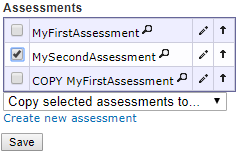
\includegraphics{images/copy-assessment.png}

\hypertarget{dummy-assessments---some-scheduling-tricks}{%
\section{Dummy assessments - some scheduling tricks}\label{dummy-assessments---some-scheduling-tricks}}

Empty assessments that doesn't contain any instruments can be used as timers to schedule administrative activities.

\textbf{Example 1, Scheduling automatic events:} A single, empty assessment can be created to hold the time point from which other assessments are scheduled to automatically become available. This circumvents the issue when a ``real'' but reoccurring assessment can't be used as starting date for a timetable.

\textbf{Example 2, Scheduling manual actions:} An empty assessment can also be used together with flagging to prompt a certain action from the therapist. This is useful when something needs to be manually sent or done by the therapist a certain number of days into treatment while participants have individual treatment start dates. The trick is achieved by creating an empty assessment (i.e.~FLAG FOR SENDING DEVICE) that is dependent on a previous assessment (i.e.~FIRST ASSESSMENT) and activated with a chosen delay (i.e.~63 days after). By checking the box Flag participant when assessment becomes activated, the therapist will see individually occurring flags on participants whenever it is time for them to receive the attention/service from the therapist. Since the assessment doesn't contain any instruments, only the therapist will get a notice (flag).

\textbf{Example 3, Scheduling text messages (SMS):} An empty assessment that is managed In group and linked to a text message can be used to schedule an independent reminder to all participants (i.e. ``Happy New Year! If you find it hard to keep to your new lifestyle during events like this, log in and re-read the advice in module 3''). An empty assessment can also be created to remind a single individual that hasn't done so for a while to log in.

\hypertarget{assessment-instruments}{%
\section{Assessment instruments}\label{assessment-instruments}}

All available instruments are listed in the right panel of the Assessment view. To include an instrument, check the box to the left of its name and then press the \emph{Save} button. The number shown between the brackets to the right of each instrument name shows how many questions the instrument contains. The \emph{Total number of items} top row shows the current total sum of questions in the assessment.

The order in which the instruments appear in the assessment will be the same as the order they are presented in the box Assessment Instruments shown to the right. You can change the order of an instrument listed in the box by pressing the upward arrow to the left of the instrument name.

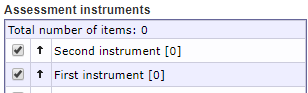
\includegraphics{images/assessment-instrument.png}

\begin{quote}
\textbf{Hint:} If you can't see any/all arrows, first select the instruments you want to include and press Save. Then change the order of the instruments and press Save again
\end{quote}

\hypertarget{participants}{%
\chapter{Participants}\label{participants}}

The ``Participants'' view is one way to access participant information. It is very similar to the ``Participant search'' view, and it is mostly down to personal preference on which to use. You can customize ``Participant search'' to show exactly the data you want to see, while ``Participants'' is predefined and more simplistic. One important difference remains, however: the \textbf{``Groups''} tab, which only exists under ``Participants''.

Depending on which project is selected in the dropdown in the main menu, the result in the ``Participants'' view will differ. If a specific project is selected, only participants in that project wil be shown under each tab.

In ``Participants'', there are four tabs:

\begin{itemize}
\tightlist
\item
  \emph{My participants}, which shows you any participants assigned to you (as a therapist)
\item
  \emph{Supervisions}, which is similiar to ``Supervised participants''
\item
  \emph{All participants}, which shows you all participants in a project. If no project is selected, it will show all participants in the database.
\item
  \emph{Groups}, which shows you the groups created in a project, and gives you the tools to manage them.
\end{itemize}

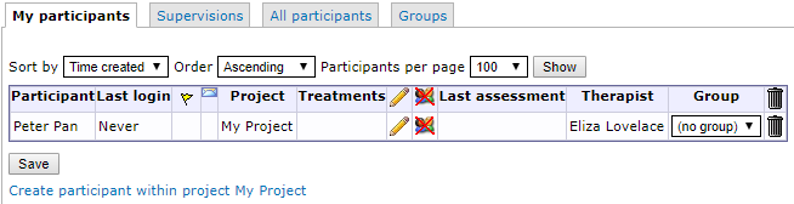
\includegraphics{images/new-images/participantsTabs.png}

\hypertarget{creating-deleting-and-editing-participants}{%
\section{Creating, deleting and editing participants}\label{creating-deleting-and-editing-participants}}

You can create new participants in two of the tabs in the Participants view; \emph{My participants} and \emph{All participants}. Participants that are created in the \emph{My participants} tab will be tagged as your participants automatically, while participants created in the \emph{All participants} tab won't be tagged.
To create a new participant, click \emph{Create participant within project {[}Project Name{]}}. Newly created participants are added at the bottom of each view.

Te delete at participant, click the trash bin icon to the far right of the corresponding participant's row.

To edit a participant, click the pencil icon in the table, on the corresponding participant's row. This will take you to the ``Participant stats'' view.
If you only wish to change, or add, what group a participant belongs to, you can do so directly in the \emph{Group} column of the participant table by using the dropdown. When you've assigned a participant to a group this way, don't forget to click the ``Save'' button at the bottom of the table.

\hypertarget{the-participant-view}{%
\section{The participant view}\label{the-participant-view}}

When you create or edit a participant, the participant view is shown. To exit this view, and return to the participants table, click the ``close'' text to the right of the participant's name. If you made any changes to the participant, don't forget to save them by clicking the ``Save'' button at the bottom of the page.

There are seven tabs in this view:

\begin{itemize}
\tightlist
\item
  \emph{Participants stats}, where you can view all fundamental information on the participant
\item
  \emph{Treatments}, where you can view and manage any treatments connected to the participant
\item
  \emph{Files}, where you can upload files relevant to the participant. These files cannot be viewed by the participant, but only by therapist who have access to the participant.
\item
  \emph{External messages}, where you can manually send SMS or e-mail messages to the participant, and review the status on any previously sent external messages.
\item
  \emph{Flags}, where you can view any flags the participant might have.
\item
  \emph{Assessments}, where you can view and manage assessments for the participant. You can also activate or deactivate individually managed assessment through this view.
\item
  \emph{Graphs}, where you can see graphs on the answers the participant has given on recurring assessments.
\end{itemize}

\hypertarget{participant-stats}{%
\subsection{Participant stats}\label{participant-stats}}

\hypertarget{instruments}{%
\chapter{Instruments}\label{instruments}}

There are two ways to create a new instrument in BASS4. Either you can copy an existing instrument, that is similar to the one you wish to create and adjust that instrument. You can also create a new instrument from scratch, using the built in tool in BASS4.

\hypertarget{copy-an-instrument}{%
\section{Copy an instrument}\label{copy-an-instrument}}

To copy an instrument, follow these steps:
1) Navigate to \textbf{Instruments} in the main menu to the left. Here you can view all instruments currently available in your database.
2) On the far right of the instrument you wish to copy, next to the trash can icon, is an icon resembling two documents. If you hover with the mouse pointer over this icon, it will say ``Copy instrument''. Clicking on this icon will create a copy of the instrument, called ``Copy of {[}Instrument{]}''.
3) Open the instrument you just created by clicking the pencil icon to the right on the instrument row. If you hover the mouse pointer over the pencil icon, it will display the tooltip ``Edit instrument''. Clicking the pencil icon will show the instrument editor. The ``Creating a new instrument'' section explains how this editor works.
4) Prior to editing the instrument, it's good practice to open a separate window or browser tab by using the \textbf{Preview-function}. This function is located under the Preview-tab, and opened by clicking the ``Open preview in Clojure app'' hyperlink. By default, a new tab will open where the instrument will be displayed in its formatted layout. It's a good idea to have this tab opened while editing the instrument in the instrument editor, and switching back and forth between the browser tabs to see your updates displayed in the Preview.

\hypertarget{creating-a-new-instrument}{%
\section{Creating a new instrument}\label{creating-a-new-instrument}}

To begin creating a new instrument, navigate to \textbf{Instruments} in the main menu on the left. This will open up a table view showing you all the instruments currently available in your database. On the bottom of the table, there is a hyperlink with the text ``Create new instrument''. Clicking this hyperlink will take you to the \textbf{General} view of the instrument editor, as shown in picture 1 below. The tabs named \textbf{Edit}, \textbf{Preview}, \textbf{Scoring Formula} and \textbf{Export} are also displayed.

\hypertarget{the-general-tab}{%
\subsection{The General Tab}\label{the-general-tab}}

This tab is where you can change the \textbf{Name} of the instrument, its \textbf{Abbreviation} (both of which are only show in the administrator's view), as well as the \textbf{Title name} (which is the title presented to the participants).
For example, this could be \textbf{Audit} in all three cases, as show in picture 1 below.

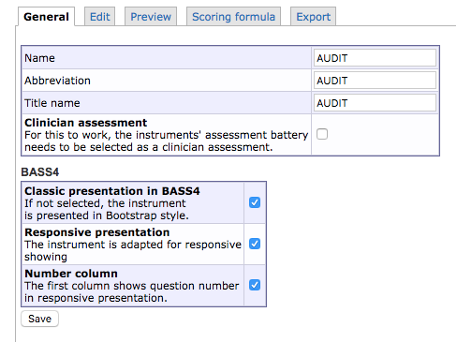
\includegraphics{images/new-images/InstrumentsGeneral1.png}
\textbf{Picture 1}

If the instrument you are creating is supposed to be filled out by a clinician, you check the box called \textbf{Clinician assessment}.

\hypertarget{the-bass4-table}{%
\subsubsection{The BASS4 Table}\label{the-bass4-table}}

This table contains three options that influence the presentation of your instrument.
\textbf{Classic presentation in BASS4} governs whether your instrument is shown in a classic layout, i.e somewhat smaller font size, or a more modern layout with a somewhat larger font size (16 pixels).
\textbf{Responsive presentation} governs whether or not your instrument is adjusted automatically according to the size of the screen it is viewed on (i.e mobile or PC/Mac). This mainly affects \emph{Question} items, where answers ordered by cell will require additional steps be taken in order to display correctly.Instructions on how to do this are found under the ``Edit'' section.
Answers ordered by line break will automatically display correctly both on mobile and PC/Mac with this option checked.
Leaving this box unchecked will cause the instrument to display its PC/Mac layout regardless of which screen it is viewed on. It will not adjust to mobile screens.
\textbf{Number column} governs whether or not the first column of the instrument is assigned to the display of question numbers in responsive presentation.

When you've entered the information, click \textbf{save}.

\hypertarget{the-preview-tab}{%
\subsection{The Preview Tab}\label{the-preview-tab}}

In this tab, you can view the instrument with it's final visual design applied (the final visual design is applied automatically by BASS) by clicking the hyperlink named ``Open preview in Clojure app''.
By default, a new tab will open, in which the instrument will be displayed with its final visual design applied. It's a good idea to have this tab opened while editing the instrument in the instrument editor, and switching back and forth between the browser tabs to see your updates displayed in the Preview.

\hypertarget{the-edit-tab}{%
\subsection{The Edit Tab}\label{the-edit-tab}}

This tab is where you create, or build, your new instrument. This is also where you adjust any instrument you've copied or want to edit. This is mainly done through adding, editing or deleting content in the form.
To begin, start by creating and defining a \textbf{table definition}

\textbf{Add table definition}
By default, the first table definition is already created. However, it has not been defined, and thus you need to define it before proceeding to adding additional items and elements to your instrument. To do this, click the ``Edit'' text in the \textbf{Table definition} box. This opens up the editor for this specific item (in this case a table definition).
One thing to note before starting to assign \textbf{Cell width} is that the total width of your instrument is fixed to 700 pixels on PC/Mac. As such, you will have to stay within those confines when defining your table definition.
If responsive presentation is used, the instrument width will adapt to a mobile screen size where applicable.

A table definition provides a layout framework for every item below it, up until the next table definition (if there is one).

A good practice is to allow the first column to take up 30 pixels of screen space. This is done by typing 30 into the first box of the \textbf{Cell width} column. If you so wish, you can justify the text of a box to be either left aligned, centered, or right aligned by choosing the corresponding option in the box's dropdown menu in the \textbf{Justify} column.
The second cell is most often reserved to the text of a question, and can be set to the desired width by typing it into the box.
Typing a * into the box makes its cell flexible, causing it to fill any left over width not claimed by the other cells in the table definition. If multiple cells are given a flexible width by typing * in their cell width boxes, they will share the left over width evenly.
The third through 16th cell is usually utlized for answers to a question item, when ordered by \textbf{Cell} (horizontally) and can be given any desired width. However, remember that width is limited if you are ordering answers by \textbf{cell}, and that long words in an answer may clip into eachother if the allocated space is too small.
Ordering answers by \textbf{line break} organizes them in a vertical structure, and as such they do not suffer this limitation. If you plan to order your answers by \textbf{line break} you only need to fill in the boxes for cell 1 and 2 in your table definition that governs the layout for the question items that utilizes \textbf{line break}

\textbf{Add information}
Usually a form starts with information on how to fill it out, and as such you want to add that information before you add your questions. To do this, click ``Add new {[}Free text{]}'' and type the information ionto the ``Free text'' box.

In ``Free text'' you type regular HTML or regular text input. You can find some basic HTML tags in the appendix of this manual, with links to more thorough resources listed as well.
In ``Layout-string'', you type {[}T{]}, which instructs BASS to render the text in the ``Free text'' box. Then press save.

\begin{quote}
\textbf{Hint:} If you want to have a line above or below your text, to act as a separator, you can type in 1 in the ``Border-width upper'' or ``Border-width lower'', respectively.
\end{quote}

\textbf{Adding questions}
Depending on what questions you would like to add, you go about adding them in different ways. We will adress the most common type of question below.

\textbf{Adding multiple-choice questions}
By follow the instructions below, your end result will look similar to this:
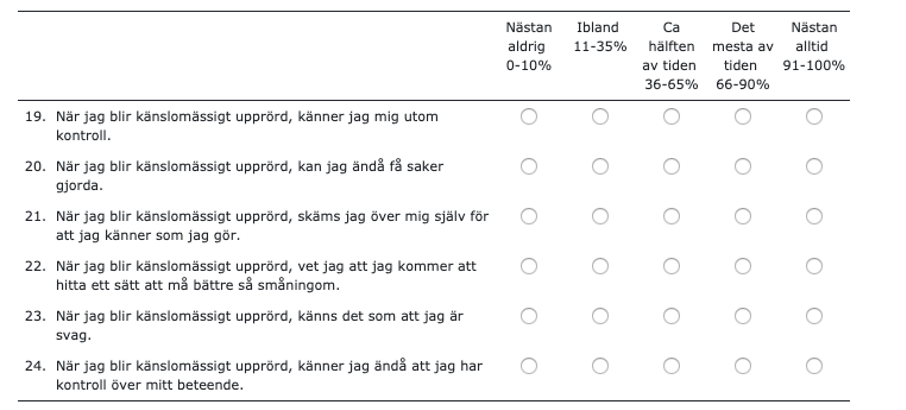
\includegraphics{images/new-images/multiplechoiceQ.png}

First, you will need to add a new ``free text''. To do this, click ``\textbf{Add new {[}Free text{]}}''. Then type in the options that are needed for the questions you want to add. For example, if you have five options to your question, you type it in like in picture 4 picture below.
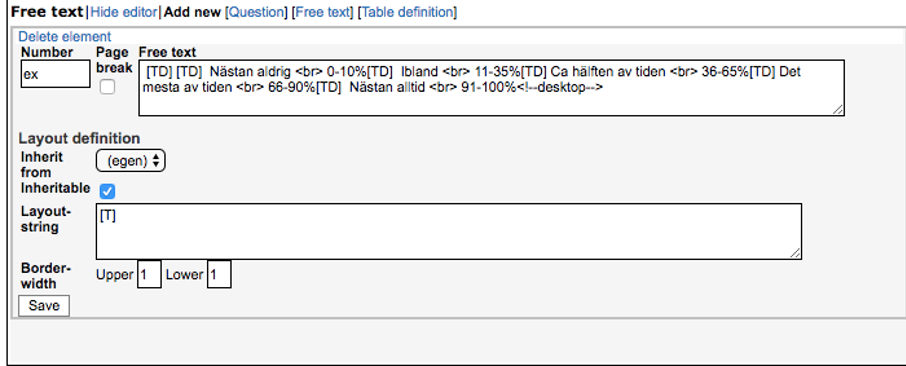
\includegraphics{images/new-images/multiplechoiceFreeText.png}
\textbf{Picture 4}

If you have more options, you add them by typing ``{[}TD{]} option 6'', before the HTML tag \texttt{\textless{}!-\/-desktop-\/-\textgreater{}}. If you have less options, you delete the superfluous {[}TD{]} with accompanying text. The reason for the twin {[}TD{]}{[}TD{]} in the beginning is to make empty space for the question you're adding later. The reason for the single {[}TD{]} between the options is to separate the options.

\begin{quote}
\textbf{Hint:} \texttt{\textless{}br\textgreater{}} is HTML and means that the rest of the text starts on a new row, i.e it implements a line break. If you want to have numbers on one row and the text under, you can add two tags in between. If it's all supposed to be on the same row, you can omit including any \texttt{\textless{}br\textgreater{}} tags.
\end{quote}

Like in the ``Free text'' example, you type {[}T{]} in ``Layout-string'' to instruct BASS to render the text. Then decide whether or not you want borders above or below the text by typing in a numerical value in ``Border-width upper'' or ``Border-width lower'', respectively. Then click ``Save''.

Below the created ``free text'', you now click ``\textbf{Add new {[}question{]}}''. In the number box, you type in the number you want to assign to the question. In the ``Question''-box you type in the question or statement.

By using the tools in the ``Answer definition'' section, you can define what type of answer you want. By default, ``\textbf{Radio buttons}'' is selected as the ``Answer type''. If you want multiple choice, you change the ``Answer type'' to ``\textbf{Checkboxes}''.
You can then fill out the different options under ``label'' (in this example you would use the same options you typed in ``free text'') and give them unique values under ``value'', see picture 5 below. The values are used to calculate the result with a scoring formula later on.

\begin{quote}
\textbf{Important note:} The values for each answer option in a question \emph{have} to be unique. If to answer options are supposed to have the same value, this is corrected for later on in the scoring formula.
\end{quote}

When you've filled in your answer options and their unique values, you can choose ``Cell'' under the ``Separator''-dropdown. In ``Layout definition'' you type in the following: \textbf{{[}N{]}.{[}TD{]}{[}Q{]}{[}TD{]}{[}X{]}}. This defines the layout for the question within the framework provided by your table definition. When this is done, click ``Save''.

\begin{quote}
\textbf{HELP! What does {[}N{]}.{[}TD{]}{[}Q{]}{[}TD{]}{[}X{]} mean?}
\end{quote}

\begin{quote}
\begin{itemize}
\tightlist
\item
  {[}N{]} Renders the number of the question in a cell. The period simply puts a period after the rendered number.
\item
  {[}TD{]} Creates an empty cell
\item
  {[}Q{]} Renders the text of the ``Question'' box in a cell
\item
  {[}X{]} Renders the answer options in a cell
\end{itemize}
\end{quote}

The input in the ``layout definition'' box is read from left to right, and is applied in the same order. In the layout above {[}N{]} is rendered in the first cell, {[}TD{]} creates a space, {[}Q{]} is rendered in the second cell and {[}X{]} is rendered in the third through seventh cell.

\begin{quote}
\textbf{Hint:} Make a habit of going back to your Preview page to see what your form looks like. This lets you correct mistakes and make adjustments as you go along.
\end{quote}

\begin{quote}
\textbf{Hint:} You can read about ``optional'', ``inheritable'', ``jump'', and ``specification text'' under ``Extra information''.
\end{quote}

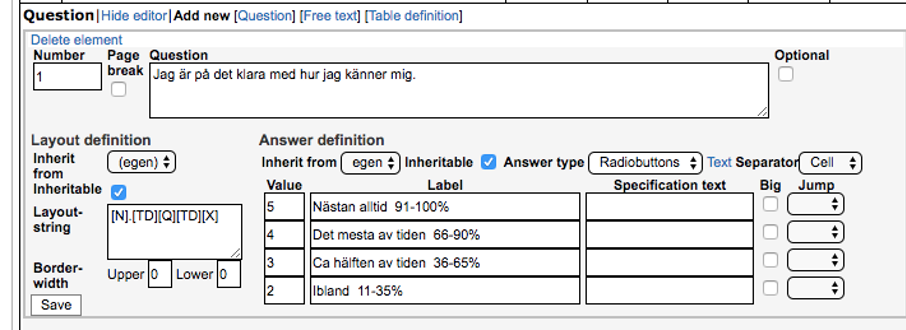
\includegraphics{images/new-images/multiplechoiceQuestion.png}
\textbf{Picture 5}

\textbf{Adding a text-answer question}
To add a question with a text answer, click ``\textbf{Add new {[}question{]}}''. Follow the same procedure as detailed above, by typing the number you want to assign to the question in the number box, and typing your question or statement into the question-box. Under ``Answer definition'', choose what type of answer you want, either ``short free text'' or ``long free text''. In ``Layour-string'', type in \textbf{{[}N{]}.{[}TD{]}{[}Q{]}{[}X{]}}.

\textbf{Having the multiple-choice answer options listed vertically instead of horizontally}
If you would rather have your answer options listed vertically below your question, you type the question in a Free text. To do this, click ``\textbf{Add new {[}Free text{]}}''. Then type the question into the free text box, and type \textbf{{[}T{]}} into the layout-string box.
Below the ``free text'' you just created, click ``\textbf{Add new {[}question{]}}''. In the number box, assign the number you wish your question to have. Leave the ``question''-box empty.
Proceed to fill out the ``Answer definition'', and type in your answer options and their unique values. Then, choose ``Line break'' in the Separator-dropdown.

\hypertarget{extra-information}{%
\subsection{Extra information}\label{extra-information}}

\textbf{Optional questions}
If the question is not mandatory, you can tell BASS to treat it as such by checking the ``optional''-box, in the upper right corner of the question-editor window. This enables a participant to complete the form without submitting an answer to that specific question.

\textbf{Page break}
If you want a question to appear on a new page, you can tell BASS to divide your form into pages by checking the ``page break''-box in the upper left corner of an editing window. By checking this box, the item for which you check it will be the first item to display on the new page. The following items will show on the new page.

\textbf{Using the jump function}
If you want an answer option to skip a participant ahead in your form, for example if a subset of questions isn't relevant if a particular answer option is selected, you can do so by using the ``jump''-function. You find this function to the right of each answer option. Open the dropdown, and select the item you wish that answer option to skip ahead to.

\textbf{Re-use layout and options}
If you have multiple questions that use the same layout and/or the same options, you can check the ``inheritable''-boxes for ``layout-string'' and/or ``answer options''. This enables the settings of one question to be inherited by another. In the editing window of the questions you wish to be inheriting settings, use the ``Inherit from''-dropdown and choose the question you want them to inherit from.

\textbf{Adding more questions}
\emph{Adding a multiple-choice question that have the same options as the previous question}.
If you want to add more questions with the same options as the previous question you just created, click ``\textbf{Add new {[}question{]}}'' and fill out the new question like you did the previous one.

\begin{quote}
\textbf{Hint:} Don't forget that you can use the ``inherit''-function. Read more about this function in the ``Extra information''-section, ``Re-use layout and options''.
\end{quote}

\emph{Adding a multiple-choice question that do not have the same options as the previous question}.
If your next question has a different set of answer options than the previous one, but the same number of answer options, you add a new free text and write the options like previously instructed, and then add the new question.

If your next question has a different \textbf{number} of options as the previous question, you need to add a new ``table definition'' that provides a new layout framework that fits the structure of the new question. Then proceed to add the new free text and question as previously instructed.

\emph{Adding a text-answer question}.
Create a new question by clicking ``\textbf{Add new {[}question{]}}'' and fill it out like previously instructed.

\hypertarget{scoring-formula}{%
\section{Scoring formula}\label{scoring-formula}}

In the \textbf{Scoring formula} tab, you can define formulas that calculate the scores from the different items in your instrument. You refer to specific items in your instrument by using the \texttt{@\#} identifier, i.e \texttt{@1} refers to question 1, \texttt{@2} refers to question 2, and so on.
Should you leave the scoring formula blank, you will still get all value readouts from your instrument. The scoring formula is meant to help with calculating different scores that are relevant to your instrument.

\begin{quote}
\textbf{Defining a calculation:} \texttt{sum\ =\ @1\ +\ @2\ +\ @3\ +\ @4\ +\ @5}
\texttt{\#sums\ sum}
\end{quote}

If you want to calculate several sums or products, you define each score (\texttt{sum}) by giving it a number.

\begin{quote}
\textbf{Adding several scores:} \texttt{sum1\ =\ @1\ +\ @2\ +\ @3}\texttt{sum2\ =\ @4\ +\ @5\ +\ @6}\texttt{sum3\ =\ @7\ +\ @8\ +\ @9}\texttt{\#sums\ sum1,\ sum2,\ sum3}
\end{quote}

\begin{quote}
\textbf{Multiplying several scores:} \texttt{sum1\ =\ (@1\ *\ @2)\ +\ (@3\ *\ @4)} \texttt{sum2\ =\ (@5\ *\ @6)\ +\ (@7\ *\ @8)} \texttt{\#sums\ sum1,\ sum2}
\end{quote}

You can also calculate the mean of a score, by dividing the number of questions included.

\begin{quote}
\textbf{Calculating the mean of a score:} \texttt{sum1\ =\ @1\ +\ @2\ +\ @3\ +\ @4\ +\ @5} \texttt{mean1\ =\ @1\ +\ @2\ +\ @3\ +\ @4\ +\ @5\ /\ 5}\texttt{\#sums\ sum1,\ mean1}
\end{quote}

Just as you can calculate several sums and products, you can also calculate several means.

\begin{quote}
\textbf{Calculating several means:} \texttt{mean1\ =\ (@1\ +\ @2\ +\ @3)\ /\ 3} \texttt{mean2\ =\ (@4\ +\ @5)\ /\ 2} \texttt{mean3\ =\ (@6\ +\ @7\ +\ @8\ +\ @9)\ /\ 4} \texttt{\#sums\ mean1,\ mean2,\ mean3}
\end{quote}

\hypertarget{create-new-treatment}{%
\chapter{Create new treatment}\label{create-new-treatment}}

BASS is designed to allow you to conduct mental healthcare and psychological studies through online channels. The main feature to achieve this in BASS, is the treatment.
A treatment is built by combining \emph{treatment modules} into sections. A module is in essence a website, contained within the framework that BASS provides. This allows you the flexibility to build your treatment according to your organization's needs and wishes.

\hypertarget{references}{%
\chapter{References}\label{references}}

\bibliography{bibliography.bib,packages.bib}

\end{document}
